
%-------------------------------------------------------------------------------------------
%%%%%%%% PREAMBLE
%-------------------------------------------------------------------------------------------
\documentclass[11pt]{article}

% Load packages
\usepackage[T1]{fontenc}

\usepackage{aeguill}
\usepackage{fancyhdr, amssymb, amsmath, geometry,setspace,lastpage,pdflscape}
\usepackage[pdftex]{graphicx,color}
\definecolor{dkblue}{rgb}{0,0.08,0.45}
\usepackage[pdftex]{hyperref}
\hypersetup{colorlinks}%
%citecolor=black,%
%filecolor=black,%
%linkcolor=black,%
%urlcolor=black}

%\usepackage{lmodern}
\usepackage{helvet}
\renewcommand{\familydefault}{\sfdefault}

% Page Setup
\geometry{ top = 1in, bottom = 1in , left=1in, right=1in}
\pagestyle{empty}
\lhead{}
\chead{}
\rhead{}
\lfoot{}
\cfoot{\footnotesize \thepage  { /}  \pageref{LastPage}}
\rfoot{}

% Paragraph Setup
\setlength{\parskip}{\baselineskip}%
\setlength{\parindent}{0pt}%

% Title Information
\title{}
\author{}
\date{}

%-------------------------------------------------------------------------------------------
%%%%%%%% DOCUMENT BEGINS HERE
%-------------------------------------------------------------------------------------------
\begin{document}

\begin{center}
{\Large Main Text Figures}
\end{center}

%-------------------------------------------------------------------------------------------
% Figure 1 - Mauke results
%-------------------------------------------------------------------------------------------
\begin{figure}[htbp]
\begin{center}
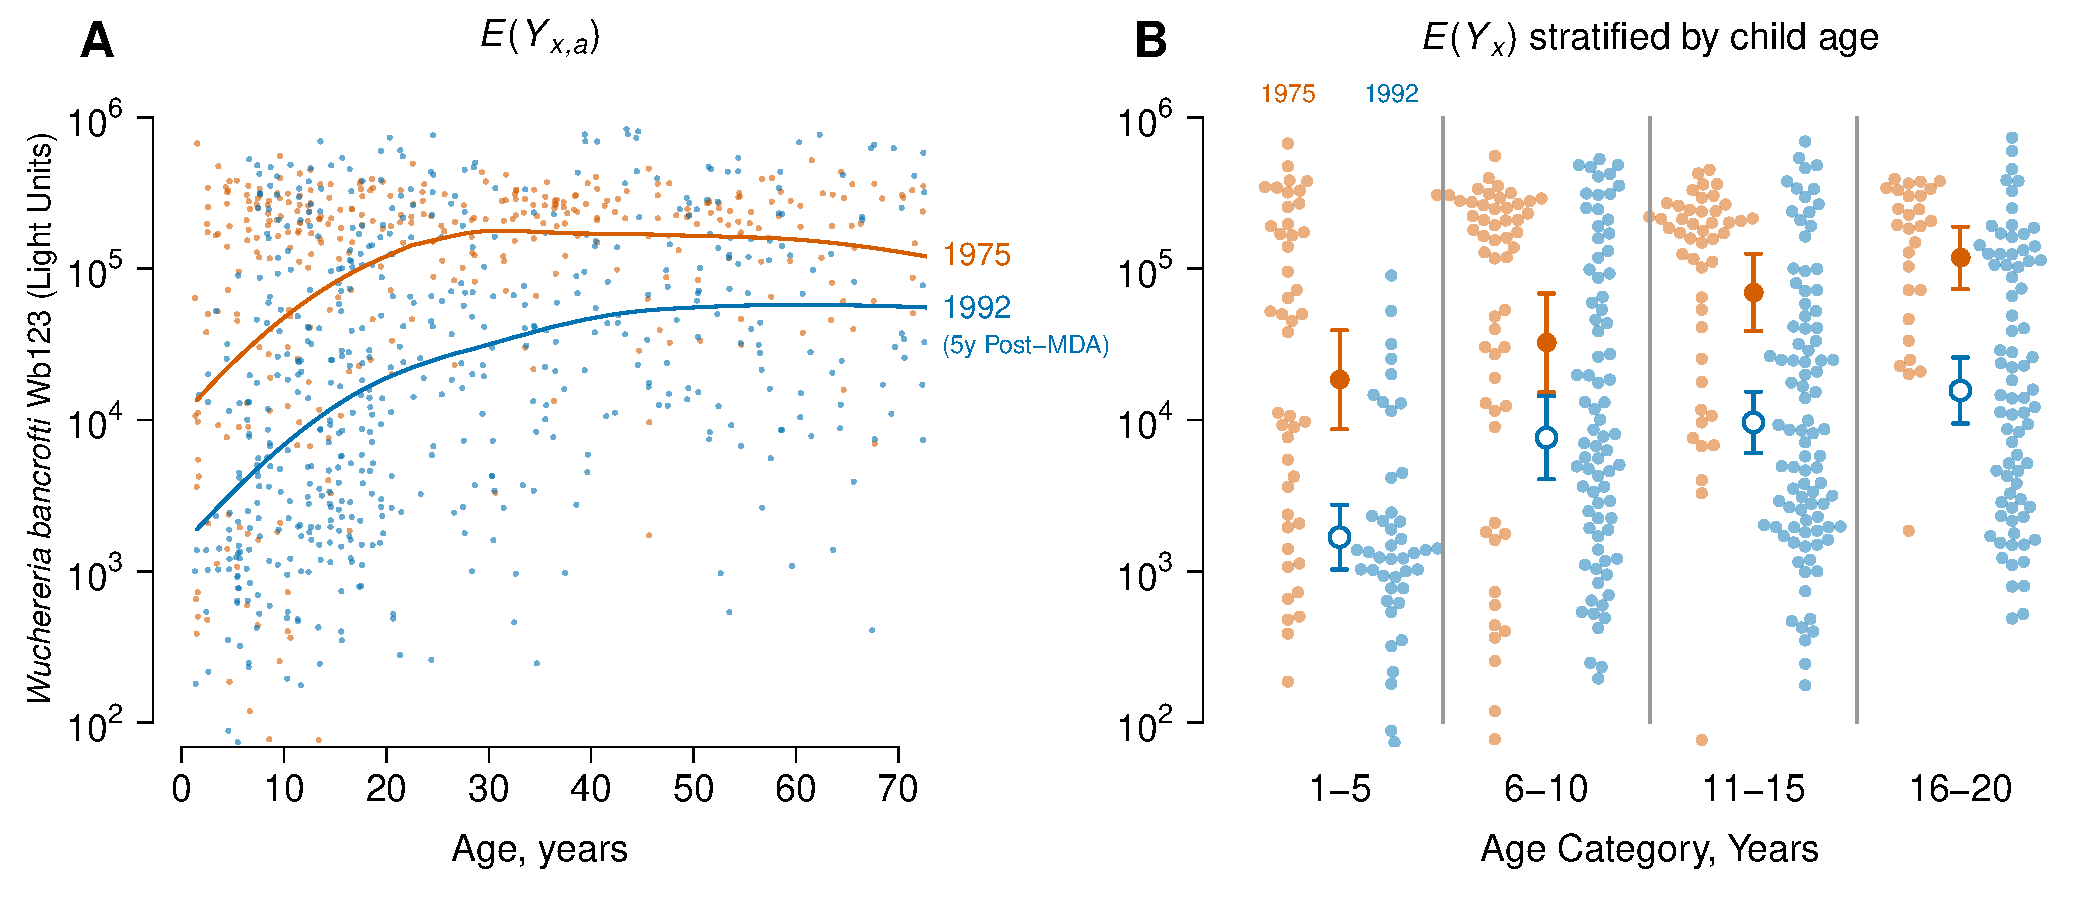
\includegraphics[width=\textwidth]{/users/benarnold/SLAbcurves/results/figs/mauke-Wb123-analysis.pdf}
\begin{minipage}{\textwidth}
\caption{Age-specific antibody response curves illustrating a shift in transmission intensity of \textit{Wuchereria bancrofti} due to mass drug administration (MDA) on Mauke Island.  Antibody response to the Wb123 antigen for \textit{W. bancrofti} measured in blood specimens with a luciferase immunoprecipitation system assay from residents in 1975 (N=362) before MDA and again in 1992 (N=553), five years following a single, island-wide MDA with diethylcarbamazine. \textbf{A.} The figure includes mean antibody levels $E(Y_{x,a})$ by group ($x$) and age ($a$) for ages 0-70 years; individual antibody responses (points) are shown along with summary curves fit with an ensemble machine learning algorithm (Online Methods). \textbf{B.} Beeswarm plots show individual antibody responses by survey (pre- vs. post-MDA) and age category; circles with error bars illustrate group-specific geometric mean antibody levels $E(Y_{x})$ and their 95\% confidence intervals, stratified by age category (all differences significant at $P\leq0.01$ after Bonferroni correction).  }
\label{fig:mauke}
\end{minipage}
\end{center}
\end{figure}


%-------------------------------------------------------------------------------------------
% Figure 2 - Garki results
%-------------------------------------------------------------------------------------------

\begin{figure}[htbp]
\begin{center}
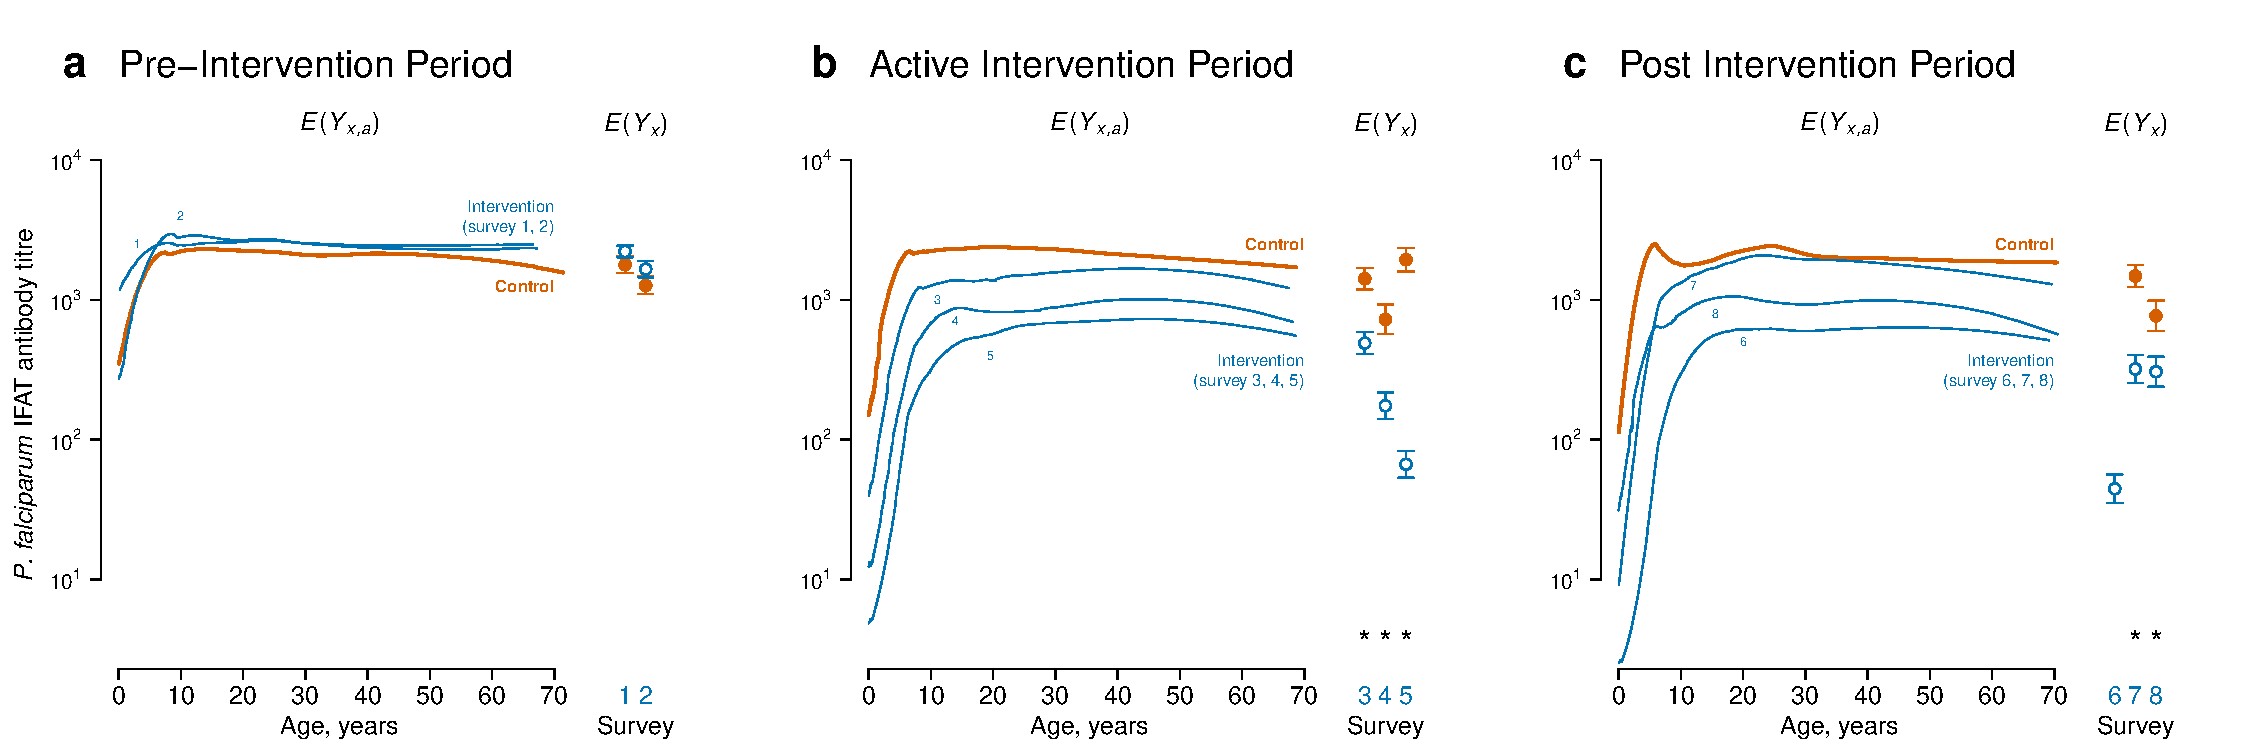
\includegraphics[width=\textwidth]{/users/benarnold/SLAbcurves/results/figs/garki-antibody-curves-IFATPf.pdf}
\begin{minipage}{\textwidth}
\caption{Age-specific antibody response curves measure changes in malaria transmission due to intervention in the Garki Project, Nigeria (1970-1976). Antibody response measured with the immunofluorescence antibody test (IFAT) for \textit{Plasmodium falciparum}. \textbf{A.} pre-intervention period (survey rounds 1-2); \textbf{B.} active intervention period (survey rounds 3-5, at 20, 50, and 70 weeks following the start of intervention); \textbf{C.} post-intervention period (survey rounds 6-8 at. xxx, xxx, and xxx weeks following the end of the intervention).  Age-specific antibody curves, $E(Y_{x,a})$ by group ($x$) and age ($a$), were estimated nonparametrically from quantitative antibody responses in individuals (N=6,024) using an ensemble machine learning algorithm (Online Methods). Control measurements were combined across survey rounds within each period when plotting the curves to facilitate visual comparison of shifts in transmission intensity between surveys. Age-adjusted geometric means by group, $E(Y_x)$, provide summary differences between curves at each survey round. Error bars show 95\% confidence intervals for the age-adjusted geometric means and asterisks indicate $P\leq0.01$ (Bonferroni corrected) for differences between control and intervention groups. Control villages were not measured in survey 6.  }
\label{fig:garki}
\end{minipage}
\end{center}
\end{figure}

%-------------------------------------------------------------------------------------------
% Figure 3 - Enterics
%-------------------------------------------------------------------------------------------

\begin{figure}[htbp]
\begin{center}
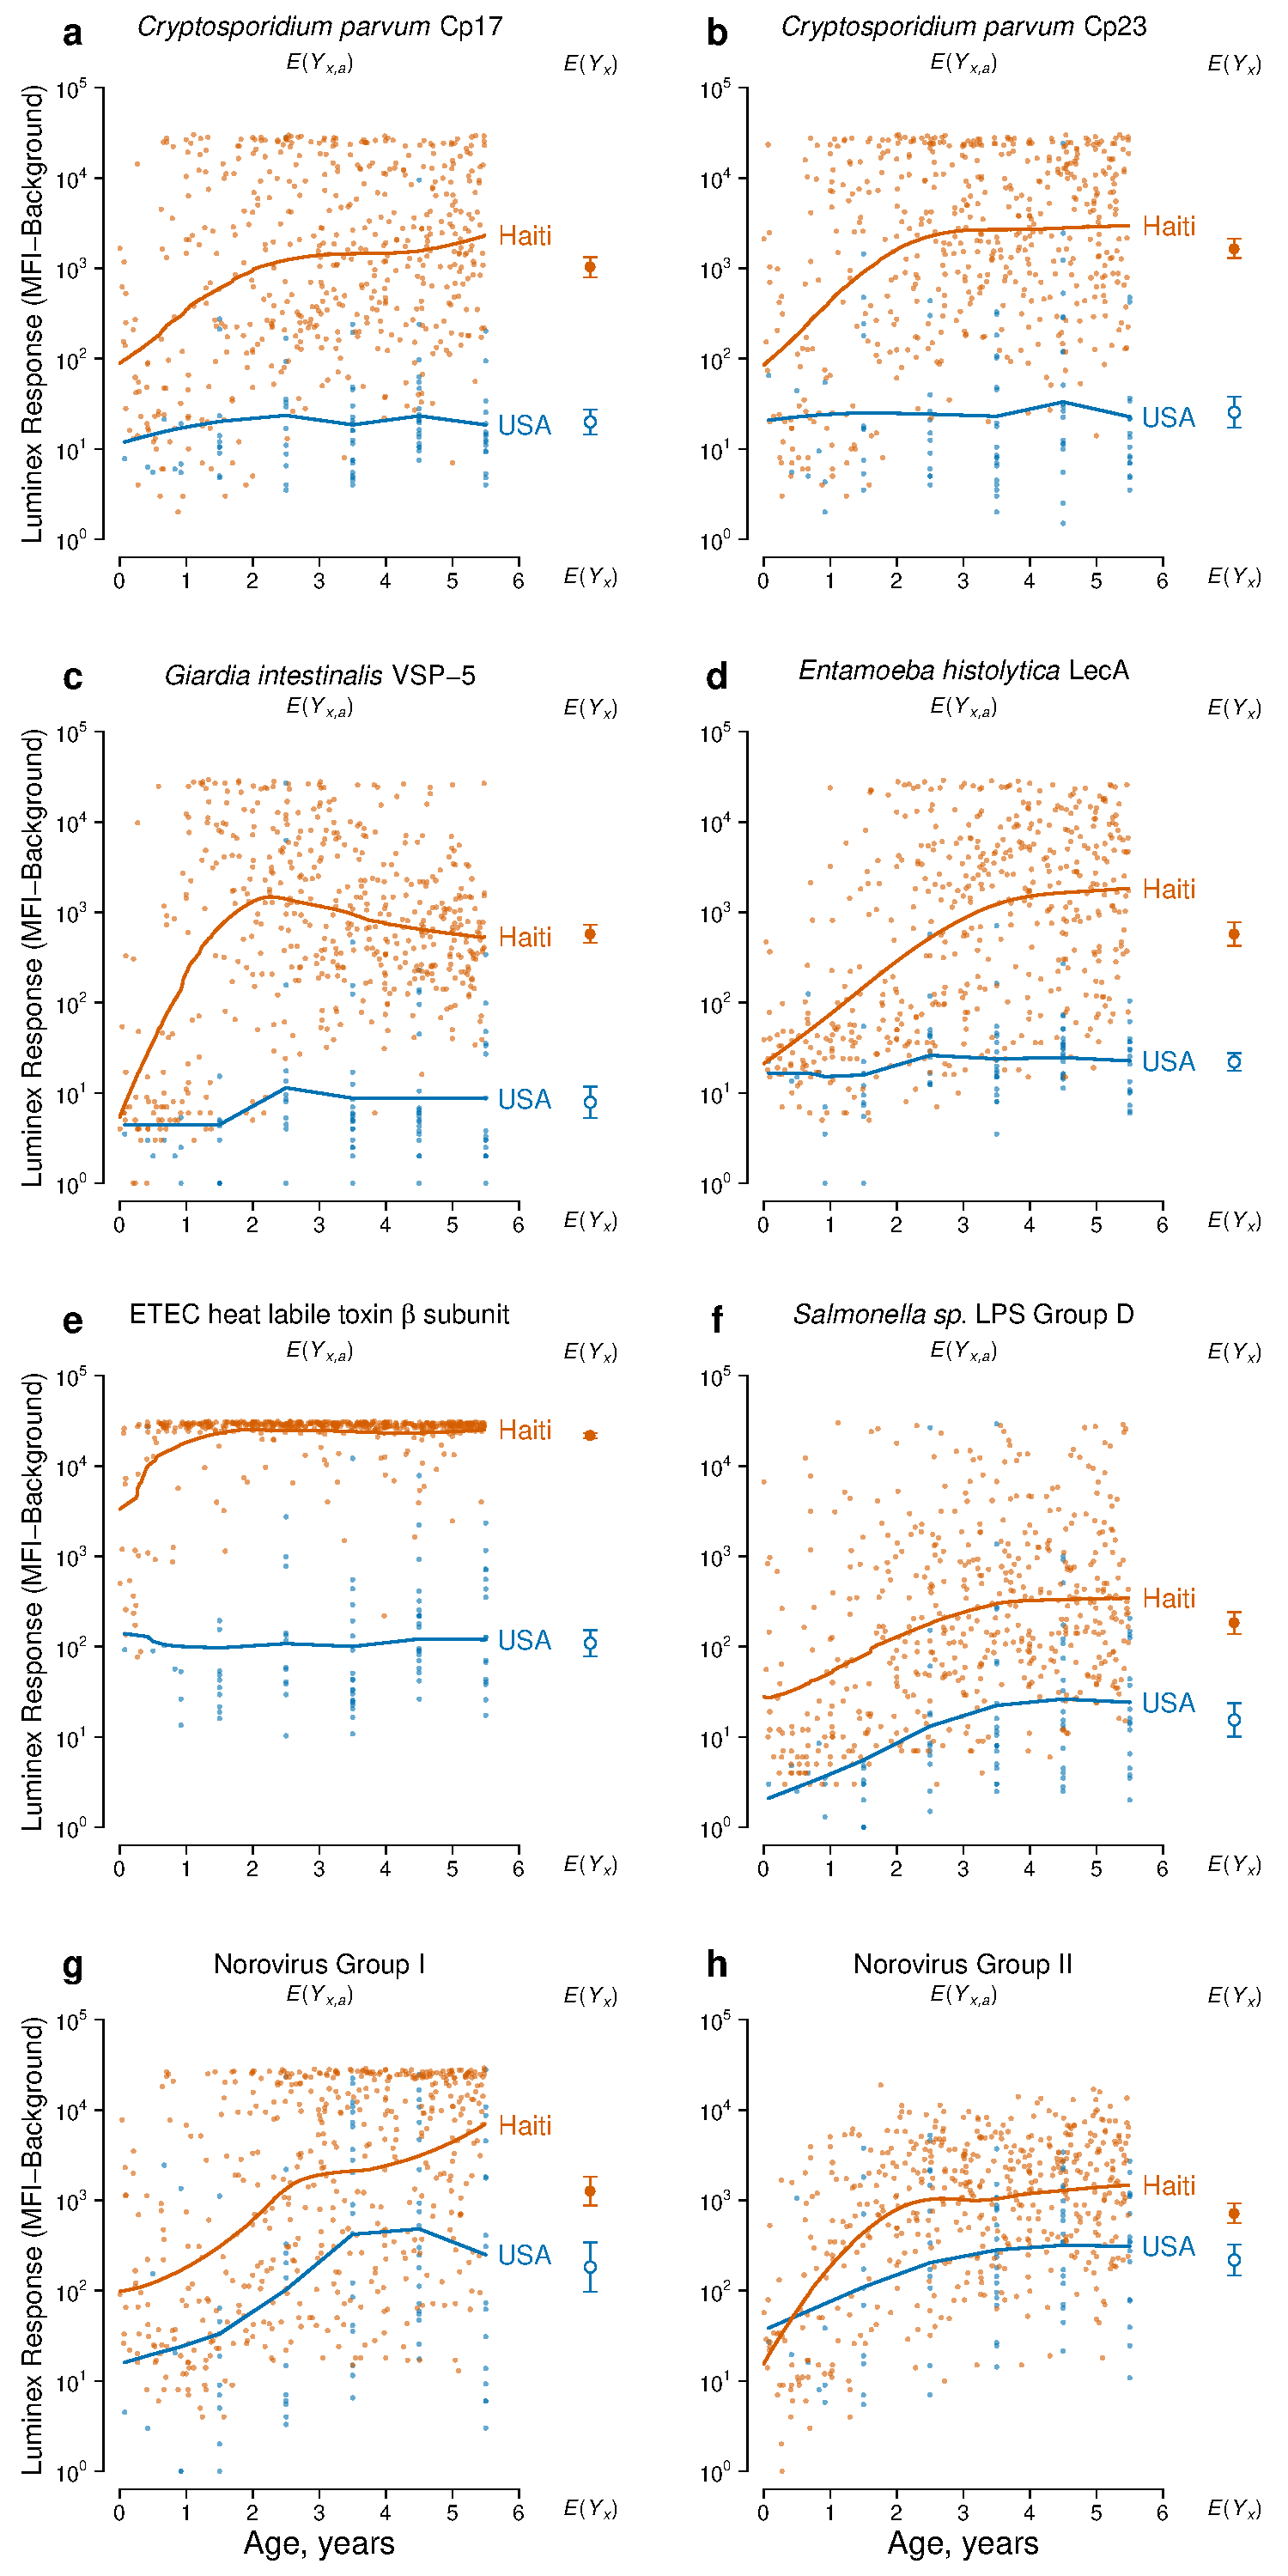
\includegraphics[width=0.7\textwidth]{/users/benarnold/SLAbcurves/results/figs/haiti2-USA-enterics-SL-curves.pdf}
\begin{minipage}{\textwidth}
\caption{caption on the next page}
\label{fig:enterics}
\end{minipage}
\end{center}
\end{figure}

\clearpage
Figure 3: Differences in enteric pathogen transmission between children in Leogane, Haiti (N=511) and the United States (USA) (N=86) measured by age-specific antibody response curves. Antibody response measured as median fluorescence intensity (MFI) minus background in multiplex bead assays on the Luminex platform. In each panel, individual antibody responses (points) are shown along with age-specific summary curves, $E(Y_{x,a})$, by country ($x$) and age($a$), fit with an ensemble machine learning algorithm (Online Methods). Each panel also includes the geometric mean by country, $E(Y_{x})$, with error bars indicating 95\% confidence intervals (all differences significant at $P\leq0.01$ after Bonferroni correction).
\textbf{A.} \textit{Cryptosporidium parvum} recombinant 17-kDa antigen;
\textbf{B.} \textit{Cryptosporidium parvum} recombinant 27-kDa antigen;
\textbf{C.} \textit{Giardia intestinalis} variant-specific surface protein-5 (VSP-5);
\textbf{D.} \textit{Entamoeba histolytica} lectin adhesion molecule (LecA);
\textbf{E.} enterotoxigenic \textit{Escherichia coli} (ETEC) heat labile toxin $\beta$ subunit;
\textbf{F.} \textit{Salmonella sp.} lipopolysaccaride (LPS) Group D;
\textbf{G.} Norovirus Group I (xx additional details needed);
\textbf{H.} Norovirus Group II (xx additional details needed).

%-------------------------------------------------------------------------------------------
% Supporting information figures
%-------------------------------------------------------------------------------------------
\clearpage
\begin{center}
{\Large Supporting Information Figures}
\end{center}

\end{document}